\section{Čvorovi naredbi}
\label{sec:MyASTStatementNodes}

Naredbe su najkomplikovanije za apstrahovanje zbog njihove raznovrsnosti. Programski jezici često uvode nove sintaksne strukture i naredbe koje nisu do tada viđene u ostalim jezicima. Uprkos svemu tome, ipak je moguće uočiti neke sličnosti sa već postojećim konceptima i svesti ih na isti nivo. Na slici \ref{fig:StatementNodes} se mogu videti tipovi apstraktnih konstrukcija koje će se koristiti da bi se predstavile naredbe.

\begin{figure}[h!]
\centering
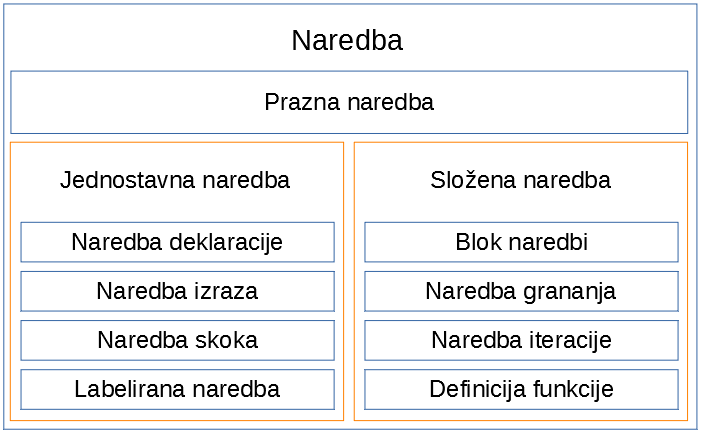
\includegraphics[scale=0.5]{images/statement_nodes.png}
\caption{Vrste čvorova naredbi.}
\label{fig:StatementNodes}
\end{figure}

Veliki broj programskih jezika podržava praznu naredbu, sa semantikom ne izvršavanja nikakvih operacija. U programskim jezicima koji su zasnovani na sintaksi jezika C, praznu naredbu navodimo samo korišćenjem simbola za kraj naredbe (\texttt{;}), dok u programskom jeziku Python koristimo ključnu reč \texttt{pass}. 

Naredbe su podeljene na \emph{jednostavne} i \emph{složene}, koje se sastoje od više drugih naredbi. Primer jednostavne naredbe može biti deklaracija promenljive, dok primer složene naredbe može biti definicija funkcije koja se sastoji od više jednostavnih deklaracija ali možda i drugih složenih naredbi kao što su grananja i petlje.

Jednostavne naredbe uključuju naredbe deklaracije i izraza. Razlog zašto se deklaracije i izrazi opet pojavljuju je taj što izrazi sami po sebi mogu biti deo drugih naredbi. Ukoliko se naredba sastoji samo od izraza, onda nju zovemo naredbom izraza. Primer može biti izraz dodele --- vrednost izraza dodele se može koristiti u drugim izrazima ali, ukoliko samo želimo da izvršimo dodelu i ništa više u okviru iste naredbe, onda izraz dodele "umotavamo" u naredbu izraza. Slično važi i za deklaracije, ukoliko razmotrimo idiomsku \texttt{for} petlju (od standarda C99) --- moguće je deklarisati promenljive koje se koriste unutar ciklusa ali to nije naredba deklaracije već deklaracija koja se koristi unutar druge naredbe. 

Naredbe se mogu označiti, po uzoru na koncept \emph{labele} u imperativnim jezicima --- identifikatora koji označava lokaciju u izvornom kodu. Labele se u imperativnim jezicima najviše koriste da bi se izvršili skokovi na određene lokacije u kodu ali su takođe prisutne i u proceduralnim jezicima (npr. kroz naredbu višestrukog grananja --- \texttt{switch} ili u nekim jezicima \texttt{case}). Labelirana naredba se sastoji od naredbe i identifikatora koji predstavlja labelu. 

Naredbe skoka se koriste obično u paru sa labeliranim naredbama, ali to ne mora uvek biti slučaj. Iako ove čvorove koristimo da bismo predstavili naredbe skoka prisutne u imperativnim jezicima, one predstavljaju i naredbe prekida (\texttt{break} ili \texttt{continue}) ili povratka vrednosti funkcije (\texttt{return}). U slučaju da je u pitanju skok na određenu labelu, onda se sastoji i od identifikatora koji predstavlja labelu na koju se skače. Ukoliko je u pitanju naredba prekida, nisu potrebne nikakve dodatne informacije (mada se i u tom slučaju može iskoristiti činjenica da su u pitanju skokovi pa se može labelirati petlja na koju se odnosi naredba prekida). U slučaju povratka vrednosti funcije, sadrži opcioni izraz čija vrednost predstavlja povratnu vrednost funkcije.

Složene naredbe se sastoje od više drugih naredbi (ne nužno samo od jednostavnih). Često je potrebno izvršiti više naredbi u okviru jednog konteksta i za to se koristi blok naredba. Blok naredba grupiše više drugih naredbi u jednu. Blok naredba se u proceduralnim jezicima obično navodi eksplicitno, za programski jezik C pomoću velikih zagrada (\texttt{\{\}}), a za skript jezike često je implicitna ili se navodi korišćenjem različitih nivoa indentacije (Python).

Naredbe uslovnog grananja se sastoje od \emph{uslova}, koji može biti relacioni ili logički izraz, naredbe koja se vrši ukoliko je uslov ispunjen (\emph{then} grama), i opciono naredbe koja se izvršava ako uslov nije ispunjen (\emph{else} grana). Rezultat uslovnog izraza, iako mora biti istinitosna vrednost, je dozvoljeno da bude bilo kog tipa (dakle nema ograničenja samo na relacione i logičke izraze) iz razloga što određeni programski jezici dozvoljavaju automatsku konverziju brojevnih tipova u logički (C). Štaviše, nekada je moguća i implicitna konverzija određenih tipova u logički tip definisanjem implicitnih operatora konverzije (C\#). Zato će u apstrakciji uslov biti bilo koji izraz. Što se \emph{then} i \emph{else} grana tiče, one mogu biti bilo koje naredbe, ali zarad konzistentnosti će obe biti blokovi naredbi. Na slici \ref{fig:MyASTExampleStatement} se može videti AST za naredbu grananja.

\begin{figure}[h!]
\begin{lstlisting}
do                               something()
    something()                  while (condition) do
while (condition)                    something()
\end{lstlisting}
\begin{lstlisting}
repeat                           something()
    something()                  while (not condition) do
until (condition)                    something()
\end{lstlisting}
\caption{Procedura svođenja ređih tipova petlji (levo) na \emph{while} petlju (desno) prikazana u pseudo-jeziku.}
\label{fig:ASTIterationStatements}
\end{figure}

Naredbe iteracije imaju raznovrsni oblik u programskim jezicima. Najčešće podržane naredbe iteracije su \emph{for}, \emph{while} i \emph{foreach} petlje. U opštem slučaju, dovoljno je koristiti samo jedan tip petlji, ali zarad jednostavnosti i prisutnosti ovih tipova u velikoj većini programskih jezika oba će biti podržana. Ostali tipovi petlji, kao što su \emph{do-while} ili \emph{repeat-until} petlje, će se svoditi na njih. \emph{do-while} petlja se može svesti na \emph{while} petlju jednostavnim ponavljanjem tela petlje pre same petlje i kreiranjem obične \emph{while} petlje sa istim uslovom i telom. Slično se može uraditi i za \emph{repeat-until} petlju, s tim što je potrebno samo negirati uslov u dobijenoj \emph{while} petlji. Ovaj proces je ilustrovan na slici \ref{fig:ASTIterationStatements}.

\begin{figure}[h!]
\centering
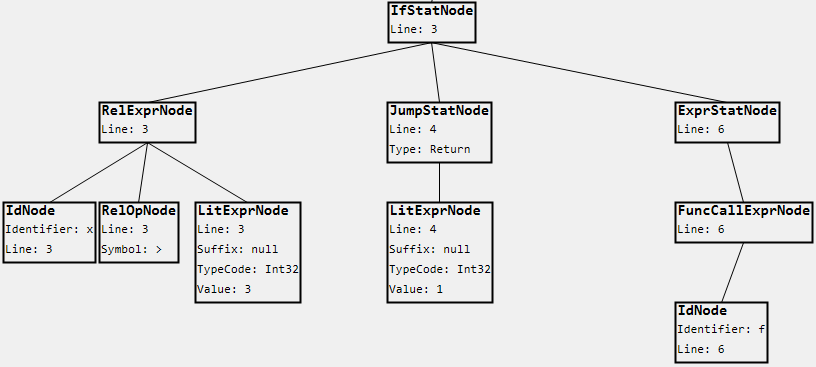
\includegraphics[scale=0.7]{images/ast_stat.png}
\caption{AST naredbe grananja.}
\label{fig:MyASTExampleStatement}
\end{figure}
